\documentclass[11pt,a4paper]{article}

% ── Packages ──────────────────────────────────────────────────────────────────
\usepackage[T1]{fontenc}
\usepackage[utf8]{inputenc}
\usepackage[left=0.7in,right=0.7in,top=0.7in,bottom=0.7in]{geometry}
\usepackage{amsmath,amssymb}
\usepackage{graphicx}
\usepackage{booktabs}
\usepackage{array}
\usepackage{tabularx}
\usepackage{caption}
\usepackage{hyperref}
\usepackage{xcolor}
\usepackage{listings}
\usepackage{float}
\usepackage{enumitem}
\usepackage{titlesec}
\usepackage{fancyhdr}
\usepackage{microtype}
\usepackage{parskip}
\usepackage{setspace}
\usepackage{tikz}
\usetikzlibrary{shapes.geometric,shapes.multipart,arrows.meta,positioning,backgrounds,fit}
\usepackage{multicol}

% ── Tighter spacing ──────────────────────────────────────────────────────────
\setstretch{0.95}
\setlength{\parskip}{4pt plus 1pt minus 1pt}
\setlist{nosep, topsep=2pt, itemsep=2pt, parsep=1pt}

% ── Section spacing ──────────────────────────────────────────────────────────
\titlespacing*{\section}{0pt}{10pt plus 2pt minus 2pt}{4pt plus 1pt minus 1pt}
\titlespacing*{\subsection}{0pt}{8pt plus 2pt minus 2pt}{3pt plus 1pt minus 1pt}
\titlespacing*{\subsubsection}{0pt}{6pt plus 1pt minus 1pt}{2pt plus 1pt minus 1pt}

% ── Caption spacing ──────────────────────────────────────────────────────────
\captionsetup{skip=4pt, font=small}

% ── Float spacing ────────────────────────────────────────────────────────────
\setlength{\floatsep}{6pt plus 2pt minus 2pt}
\setlength{\textfloatsep}{8pt plus 2pt minus 2pt}
\setlength{\intextsep}{6pt plus 2pt minus 2pt}

% ── Hyperref setup ────────────────────────────────────────────────────────────
\hypersetup{
    colorlinks=true,
    linkcolor=blue!60!black,
    citecolor=blue!60!black,
    urlcolor=blue!60!black,
}

% ── Listings (code blocks) ────────────────────────────────────────────────────
\definecolor{codebg}{HTML}{F5F5F5}
\definecolor{codecomment}{HTML}{5C6370}
\definecolor{codekeyword}{HTML}{0057AE}
\definecolor{codestring}{HTML}{007020}

\lstdefinelanguage{Java}{
  keywords={public,static,void,new,return,if,for,while,class,int,boolean,true,false,null},
  keywordstyle=\color{codekeyword}\bfseries,
  commentstyle=\color{codecomment}\itshape,
  stringstyle=\color{codestring},
  basicstyle=\ttfamily\footnotesize,
  backgroundcolor=\color{codebg},
  frame=single,
  framesep=3pt,
  rulecolor=\color{gray!40},
  breaklines=true,
  showstringspaces=false,
  tabsize=4,
  captionpos=b,
  aboveskip=4pt,
  belowskip=4pt,
}

\lstset{
  basicstyle=\ttfamily\footnotesize,
  backgroundcolor=\color{codebg},
  frame=single,
  framesep=3pt,
  rulecolor=\color{gray!40},
  breaklines=true,
  showstringspaces=false,
  tabsize=4,
  aboveskip=4pt,
  belowskip=4pt,
}

\tikzset{
  block/.style={
    rectangle, rounded corners=4pt,
    draw=blue!55!black, fill=blue!9,
    text width=#1, align=center,
    minimum height=0.68cm, font=\footnotesize,
    inner sep=3pt},
  block/.default=2.2cm,
  dbase/.style={
    cylinder, shape border rotate=90, aspect=0.28,
    draw=orange!70!black, fill=orange!14,
    text width=1.8cm, align=center,
    minimum height=0.68cm, font=\footnotesize,
    inner sep=3pt},
  result/.style={
    rectangle, rounded corners=4pt,
    draw=green!55!black, fill=green!12,
    text width=2.1cm, align=center,
    minimum height=0.68cm, font=\footnotesize,
    inner sep=3pt},
  myarrow/.style={-{Stealth[length=5pt,width=4pt]}, thick, draw=gray!60},
}

% ── Section formatting ────────────────────────────────────────────────────────
\titleformat{\section}{\large\bfseries}{{\thesection.}}{0.5em}{}[\titlerule]
\titleformat{\subsection}{\normalsize\bfseries}{{\thesubsection}}{0.5em}{}
\titleformat{\subsubsection}{\normalsize\itshape\bfseries}{{\thesubsubsection}}{0.5em}{}

% ── Header / Footer ───────────────────────────────────────────────────────────
\pagestyle{fancy}
\fancyhf{}
\fancyhead[L]{\small\textbf{CODEPROMPTZIP}}
\fancyhead[R]{\small NLP + Deep Learning Project, April 2026}
\fancyfoot[C]{\thepage}
\renewcommand{\headrulewidth}{0.4pt}

% ── Misc helpers ──────────────────────────────────────────────────────────────
\newcolumntype{L}[1]{>{\raggedright\arraybackslash}p{#1}}
\newcolumntype{C}[1]{>{\centering\arraybackslash}p{#1}}

% ══════════════════════════════════════════════════════════════════════════════
\begin{document}

% ── Title (a) ─────────────────────────────────────────────────────────────────
\begin{center}
  {\LARGE\bfseries CODEPROMPTZIP: Code-Specific Prompt Compression for Bugs2Fix}\\[0.7em]
  {\normalsize
    Ansh Gupta~(IMT2023540)\quad
    Mayank Tanwar~(IMT2023012)\quad
    Prakrititz Borah~(IMT2023547)\\
    Kunal Jindal~(IMT2023049)
  }
\end{center}

% ══════════════════════════════════════════════════════════════════════════════
% (b) Problem Definition / Scope
% ══════════════════════════════════════════════════════════════════════════════
\section{Problem Definition / Scope}

Modern LLM-based code repair pipelines use \textbf{Retrieval-Augmented Generation (RAG)}: before asking the model to fix a bug, similar buggy--fixed code pairs are retrieved from a knowledge base and placed into the prompt as demonstrations. While effective, this creates two critical bottlenecks:

\begin{itemize}[leftmargin=1.5em]
  \item \textbf{Context window limits}: retrieved examples containing full buggy and fixed methods consume thousands of tokens, often exceeding the LLM's context window.
  \item \textbf{High inference cost}: proprietary APIs charge per token, making bloated prompts prohibitively expensive.
\end{itemize}

Existing prompt compression methods (LLMLingua, RECOMP, LLMLingua-2) were designed for natural language and fail on code because they do not consider the \textbf{syntactic role} of tokens. An entropy-based approach might discard a method invocation like \texttt{.getInstance()} because its sub-tokens are predictable, even though it is semantically critical for understanding a bug.

\textbf{CODEPROMPTZIP} addresses this gap by introducing a \textbf{code-specific prompt compression framework} that leverages program analysis to understand which tokens are safe to remove for a given downstream task. This project implements and evaluates the complete CODEPROMPTZIP pipeline on the \textbf{Bugs2Fix} task, where a buggy Java method is given as input and the model must output the corrected version.

% ══════════════════════════════════════════════════════════════════════════════
% (c) Planned Approach with Justification
% ══════════════════════════════════════════════════════════════════════════════
\section{Planned Approach with Justification}

\subsection{Why CODEPROMPTZIP?}

We chose to implement CODEPROMPTZIP over alternative compression methods for three reasons:

\begin{enumerate}[leftmargin=1.5em]
  \item \textbf{Task-specific compression:} Unlike generic methods, CODEPROMPTZIP derives a token removal priority ranking specific to each downstream task (Bugs2Fix), ensuring that only tokens irrelevant to the repair signal are removed.
  \item \textbf{Controllable compression ratio:} The framework allows specifying an exact compression ratio $\tau_{\text{code}}$ at inference time via special tokens, unlike summary-based methods that produce variable-length summaries.
  \item \textbf{Copy mechanism:} The pointer-generator architecture ensures the compressed output is strictly a subset of the input tokens, no hallucinated code, which is critical for code tasks.
\end{enumerate}

\subsection{Framework Architecture}

The framework operates in two phases.

\subsubsection*{Training Phase}

\begin{figure}[H]
\centering
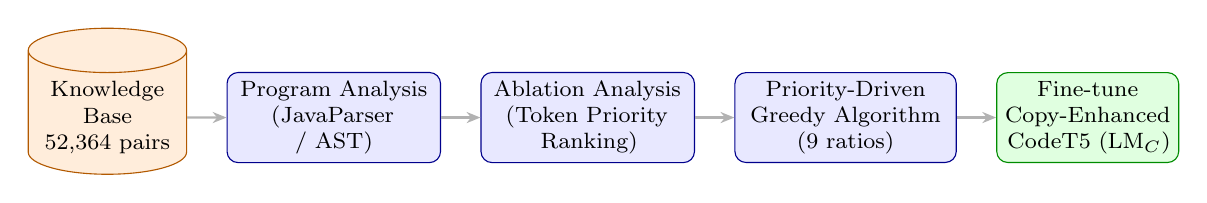
\begin{tikzpicture}[node distance=0.3cm and 0.4cm]
  \node[dbase] (kb) {Knowledge\\Base\\52,364 pairs};
  \node[block=2.5cm, right=0.5cm of kb] (pa) {Program Analysis\\(JavaParser / AST)};
  \node[block=2.5cm, right=0.5cm of pa] (ab) {Ablation Analysis\\(Token Priority\\Ranking)};
  \node[block=2.6cm, right=0.5cm of ab] (gr) {Priority-Driven\\Greedy Algorithm\\(9 ratios)};
  \node[result, right=0.5cm of gr] (ft) {Fine-tune\\Copy-Enhanced\\CodeT5 ($\text{LM}_C$)};
  \draw[myarrow] (kb) -- (pa);
  \draw[myarrow] (pa) -- (ab);
  \draw[myarrow] (ab) -- (gr);
  \draw[myarrow] (gr) -- (ft);
\end{tikzpicture}
\caption{Training pipeline: from knowledge base to fine-tuned compressor.}
\label{fig:training}
\end{figure}

\subsubsection*{Inference Phase}

\begin{figure}[H]
\centering
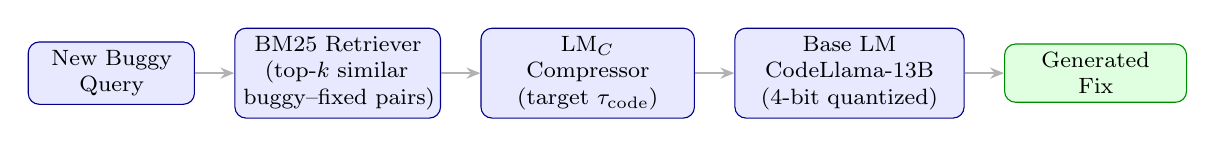
\begin{tikzpicture}[node distance=0.3cm and 0.4cm]
  \node[block=1.9cm] (q) {New Buggy\\Query};
  \node[block=2.4cm, right=0.5cm of q] (bm25) {BM25 Retriever\\(top-$k$ similar\\buggy--fixed pairs)};
  \node[block=2.5cm, right=0.5cm of bm25] (lmc) {$\text{LM}_C$\\Compressor\\(target $\tau_{\text{code}}$)};
  \node[block=2.7cm, right=0.5cm of lmc] (lm) {Base LM\\CodeLlama-13B\\(4-bit quantized)};
  \node[result, right=0.5cm of lm] (fix) {Generated\\Fix};
  \draw[myarrow] (q)    -- (bm25);
  \draw[myarrow] (bm25) -- (lmc);
  \draw[myarrow] (lmc)  -- (lm);
  \draw[myarrow] (lm)   -- (fix);
\end{tikzpicture}
\caption{Inference pipeline. $\text{LM}_C$ and the base LM are fully decoupled: compressed output is plain text.}
\label{fig:inference}
\end{figure}

The compressor ($\text{LM}_C$) and the base LM are \textbf{fully decoupled}: the compressed output is plain text, requiring no gradient sharing or special embeddings between models.

\subsection{Key Technical Components}

\subsubsection{Type-Aware Priority Ranking}

Using JavaParser to construct Abstract Syntax Trees (ASTs), every token in a code snippet is categorized into one of five types:

\begin{table}[H]
  \centering
  \caption{Token type definitions and examples}
  \label{tab:token-types}
  \renewcommand{\arraystretch}{1.15}
  \begin{tabularx}{\textwidth}{L{2.5cm} X L{4.5cm}}
    \toprule
    \textbf{Token Type} & \textbf{Definition} & \textbf{Example} \\
    \midrule
    \textbf{Symbol}     & Operators, delimiters, punctuation      & \texttt{=}, \texttt{\{}, \texttt{;} \\
    \textbf{Signature}  & Method declaration and parameters        & \texttt{public static void init(...)} \\
    \textbf{Invocation} & Function/method calls                    & \texttt{Calendar.getInstance()} \\
    \textbf{Identifier} & Variable names, class names              & \texttt{VAR\_1}, \texttt{TYPE\_1} \\
    \textbf{Structure}  & Control-flow keywords                    & \texttt{if}, \texttt{for}, \texttt{return} \\
    \bottomrule
  \end{tabularx}
\end{table}

The removal priority is computed as:

\begin{equation}
  \text{Priority}(T) = \frac{\tau_{\text{code}/T}}{d_T}
\end{equation}

where $\tau_{\text{code}/T}$ is the compression ratio achieved by removing all tokens of type $T$, and $d_T$ is the resulting CodeBLEU degradation. Higher priority means a token type saves many tokens with minimal quality loss.

\paragraph{Bugs2Fix Priority Ranking (our configuration):}

\[
\text{Identifier} > \text{Invocation} > \text{Structure} > \text{Symbol} > \text{Signature}
\]

\begin{center}
{\small (remove first $\rightarrow$ remove last)}
\end{center}

This ranking was adopted directly from the ablation study performed by the original authors, as they demonstrated it to be universally effective across different base LLMs for the Bugs2Fix task. In their ablation study, the authors systematically removed tokens of each specific type in isolation and measured the resulting percentage degradation in CodeBLEU to empirically determine which token types were safest to discard (highest priority) and which were most critical (lowest priority).

% ─────────────────────────────────────────────────────────────────────────────
\subsubsection{Dataset Construction via Priority-Driven Greedy Algorithm}

For each parsable code example in the training set, the greedy algorithm:

\begin{enumerate}[leftmargin=1.5em]
  \item Assigns each token a removal priority based on its type and within-type frequency.
  \item Computes $L_{\text{rm}} = \lfloor\tau_{\text{code}} \times L\rfloor$: the number of tokens to remove.
  \item Iteratively removes the highest-priority tokens until the budget is exhausted.
  \item Returns the compressed code as the training target.
\end{enumerate}

This is repeated for \textbf{9 compression ratios} ($\tau_{\text{code}} \in \{0.1, 0.2, \ldots, 0.9\}$), producing the following dataset:

\begin{table}[H]
  \centering
  \caption{Dataset composition (source: Microsoft CodeXGLUE Bugs2Fix)}
  \label{tab:dataset}
  \renewcommand{\arraystretch}{1.15}
  \begin{tabularx}{\textwidth}{X r}
    \toprule
    \textbf{Component} & \textbf{Count} \\
    \midrule
    Raw Bugs2Fix pairs                    & 52,364 \\
    Compression ratios per example        & 9 \\
    Total compression triples             & $52{,}364 \times 9 = \mathbf{471{,}276}$ \\
    Training split (80\%)                 & \textbf{377,020} \\
    Validation split (10\%)               & \textbf{47,128} \\
    Test split (10\%)                     & \textbf{47,128} \\
    \bottomrule
  \end{tabularx}
\end{table}

The split is performed at the code-example level (not at the triple level) to prevent data leakage, all 9 compressed versions of the same code example are assigned to the same split.

\subsubsection*{Compression Progression Example}

To illustrate the priority-driven greedy removal algorithm in action, consider how the following buggy method degrades as the compression ratio ($\tau_{\text{code}}$) increases.

\begin{lstlisting}[language=Java, caption={Original ($\tau_{\text{code}} = 0.0$) --- 0\% tokens removed}]
public static TYPE_1 init(java.lang.String name, java.util.Date date) {
    TYPE_1 VAR_1 = new TYPE_1();
    VAR_1.METHOD_1(name);
    java.util.Calendar VAR_2 = java.util.Calendar.getInstance();
    VAR_2.METHOD_2(date);
    VAR_1.METHOD_3(VAR_2);
    return VAR_1;
}
\end{lstlisting}

\begin{lstlisting}[language=Java, caption={Light Compression ($\tau_{\text{code}} = 0.3$) --- 30\% target. Redundant high-frequency \texttt{Identifier} tokens (\texttt{VAR\_1}, \texttt{VAR\_2}) begin dropping first.}]
public static TYPE_1 init(java.lang.String name, java.util.Date date) {
    TYPE_1 = new TYPE_1();
    .METHOD_1(name);
    java.util.Calendar = java.util.Calendar.getInstance();
    .METHOD_2(date);
    .METHOD_3(VAR_2);
    return ;
}
\end{lstlisting}

\begin{lstlisting}[language=Java, caption={Moderate Compression ($\tau_{\text{code}} = 0.5$) --- 50\% target. Almost all \texttt{Identifier} tokens drop. Core structural context remains intact.}]
public static TYPE_1 init(java.lang.String name, java.util.Date date) {
    = new TYPE_1();
    ;
    java.util.Calendar = java.util.Calendar;
    .METHOD_2(date);
    .METHOD_3(VAR_2);
    return ;
}
\end{lstlisting}

% ─────────────────────────────────────────────────────────────────────────────
\subsubsection{Compressor Architecture: Copy-Enhanced CodeT5}

The compressor is built on \textbf{CodeT5-base} (Salesforce, 220M parameters), an encoder-decoder transformer pre-trained on 8.35M code functions across 8 programming languages.

\paragraph{Modification 1 --- Extended Vocabulary:}
Special tokens are added to signal the task and compression ratio:

\begin{lstlisting}
<BUGS2FIX> <Ratio> 0.3 </Ratio> <Compress> {code} </Compress>
\end{lstlisting}

This enables the same model to be steered to different compression levels at inference time.

\paragraph{Modification 2 --- Copy Mechanism (Pointer-Generator):}
The critical architectural addition. At each decoding step $t$:

\begin{enumerate}[leftmargin=1.5em]
  \item The decoder produces cross-attention weights $\mathbf{a}^t$ over source positions.
  \item A context vector is computed: $\mathbf{h}^*_t = \sum_i a^t_i \cdot \mathbf{h}_i$
  \item A generation gate is computed: $p_{\text{gen}} = \sigma(W_{\text{gen}} \cdot [\mathbf{h}^*_t,\, \mathbf{s}_t] + b_{\text{gen}})$
  \item The copy distribution sums attention over matching source tokens: $P_{\text{copy}}(y) = \sum_{i:\, x_i = y} a^t_i$
  \item The final distribution blends vocabulary and copy:
\end{enumerate}

\begin{equation}
  P(y) = p_{\text{gen}} \cdot P_{\text{vocab}}(y) + (1 - p_{\text{gen}}) \cdot P_{\text{copy}}(y)
\end{equation}

This ensures the compressed output is drawn strictly from the input tokens, preventing hallucinated code. The \texttt{CopyModule} is the only component initialized from scratch; all other weights are loaded from the pre-trained CodeT5-base checkpoint.

% ══════════════════════════════════════════════════════════════════════════════
% (d) Extension / Critique of the Original Work
% ══════════════════════════════════════════════════════════════════════════════
\section{Extension and Critique of the Original Work}

\subsection*{What We Replicated}

\begin{itemize}[leftmargin=1.5em]
  \item The complete CODEPROMPTZIP pipeline: type-aware priority ranking, greedy dataset construction, copy-enhanced CodeT5 compressor, and BM25-based RAG evaluation.
  \item The compression ratio sweep experiment, confirming the non-trivial relationship between compression and downstream quality.
\end{itemize}

\subsection*{Key Differences from the Original Paper}

\begin{table}[H]
  \centering
  \caption{Comparison with the original paper}
  \label{tab:differences}
  \renewcommand{\arraystretch}{1.15}
  \begin{tabularx}{\textwidth}{L{3cm} X X}
    \toprule
    \textbf{Aspect} & \textbf{Original Paper} & \textbf{Our Implementation} \\
    \midrule
    Base LM          & GPT-3.5-turbo and Gemini-1.0           & CodeLlama-13B (4-bit quantized, local) \\
    CodeT5 variant   & CodeT5-large (770M)                   & CodeT5-base (220M) \\
    Training epochs  & 10                                    & 3 ($\sim$100 hrs on RTX 4060) \\
    Training data    & 48,903 parsable $\times$ 9 = 440K     & 52,364 total $\times$ 9 = 471K \\
    Eval.\ samples   & Full test set (6,545)                 & 100 samples (resource constraint) \\
    \bottomrule
  \end{tabularx}
\end{table}

\subsection*{Critique}

\begin{enumerate}[leftmargin=1.5em]
  \item \textbf{Base LM sensitivity:} The original paper does not deeply explore how the choice of base LM affects the utility of compressed demonstrations. Our results show that CodeLlama-13B under 4-bit quantization behaves very differently from GPT-3.5-turbo specifically, it shows much less benefit from RAG demonstrations and degrades sharply with multi-shot compressed prompts.

  \item \textbf{Compression at low $\tau$:} The $\tau=0.1$ expansion behavior (producing more tokens than the input) is a known but under-discussed limitation. The copy mechanism, while powerful, does not enforce a hard length constraint.

  \item \textbf{Evaluation scale:} The paper's results on the full test set (6,545 samples) are more statistically robust than our 100-sample evaluation, which may not capture the full distribution of bug types and complexities.
\end{enumerate}

% ══════════════════════════════════════════════════════════════════════════════
% (e) Implementation Details
% ══════════════════════════════════════════════════════════════════════════════
\section{Implementation Details}

\subsection{Hardware and Environment}

\begin{table}[H]
  \centering
  \caption{Hardware and environment specifications}
  \label{tab:hardware}
  \renewcommand{\arraystretch}{1.15}
  \begin{tabularx}{\textwidth}{L{4.5cm} X}
    \toprule
    \textbf{Component} & \textbf{Specification} \\
    \midrule
    GPU                       & NVIDIA GeForce RTX 4060 (8\,GB VRAM) \\
    System Environment        & Windows (local, RTX 4060) \\
    Compressor for Finetuning    & CodeT5-base(220M) \\
    Base LM for evaluation    & CodeLlama-13B-Instruct (Q4\_K\_M quantized, GGUF) \\
    Evaluator    & CodeBLEU \\
    Python version            & 3.12 \\
    Framework                 & PyTorch + HuggingFace Transformers \\
    \bottomrule
  \end{tabularx}
\end{table}

\subsection{Training Configuration}

\begin{table}[H]
  \centering
  \caption{Training hyperparameters}
  \label{tab:hyperparams}
  \renewcommand{\arraystretch}{1.15}
  \begin{tabularx}{\textwidth}{X r}
    \toprule
    \textbf{Hyperparameter} & \textbf{Value} \\
    \midrule
    Base model                  & Salesforce/codet5-base (220M params) \\
    Micro batch size            & 2 \\
    Gradient accumulation steps & 8 \\
    \textbf{Effective batch size}        & \textbf{16} \\
    Learning rate               & $5 \times 10^{-5}$ \\
    Number of epochs            & \textbf{3} \\
    Total training steps        & ${\sim}70{,}500$ ($23{,}500$ steps/epoch $\times 3$) \\
    \textbf{Total training time}         & \textbf{${\sim}100$ hours} \\
    \bottomrule
  \end{tabularx}
\end{table}

These hyperparameters were set to fit the model within 8\,GB VRAM. The effective batch size of 16 was achieved via gradient accumulation (micro-batch $2 \times 8$ accumulation steps).

\subsection{Compressor Fine-Tuning Results}

The CodeT5-base model was fine-tuned for 3 full epochs on the 377,020 training samples. Key observations from the training curves:

\begin{itemize}[leftmargin=1.5em]
  \item \textbf{Epoch 1:} The loss dropped dramatically from 3.67 (step 100) to 0.0284 (step 23,000), reflecting the model rapidly learning to compress code using the rich pre-trained representations from CodeT5.
  \item \textbf{Epoch 2:} The validation loss improved from 0.0284 to 0.0145, a 49\% reduction confirming that a second epoch over the large dataset was valuable.
  \item \textbf{Epoch 3:} Continued to reduce, with the final best model achieving val loss = 0.0145 at step 47,000. The loss stabilized in the 0.017--0.018 range, indicating convergence.
\end{itemize}

\begin{figure}[H]
  \centering
    \includegraphics[width=0.88\textwidth]{combined_val_loss_only.png}
  \caption{Validation loss across the full 3-epoch training run. The steep initial drop (Epoch 0--0.5) reflects rapid adaptation of pre-trained CodeT5 weights. Gold stars mark ``New Best'' checkpoints.}
  \label{fig:val-loss}
\end{figure}

The best checkpoint (lowest validation loss) was selected for all downstream evaluations.

\subsection{Evaluation Pipeline}

For evaluation, we use:

\begin{itemize}[leftmargin=1.5em]
  \item \textbf{BM25 retrieval} (whitespace tokenization) to fetch similar buggy-fixed pairs from the full 52,364 training knowledge base.
  \item \textbf{CodeT5 compressor} to compress demonstrations at the specified $\tau_{\text{code}}$.
  \item \textbf{CodeLlama-13B-Instruct} (4-bit quantized) as the base LM for code generation.
  \item \textbf{CodeBLEU} as the evaluation metric, computed across four components: N-gram match, Weighted N-gram match, Syntax match (AST), and Dataflow match.
  \item 100 randomly sampled test examples (seed=42) for each experiment configuration.
\end{itemize}

% ══════════════════════════════════════════════════════════════════════════════
% (f) Results and Discussion
% ══════════════════════════════════════════════════════════════════════════════
\section{Results and Discussion}

\subsection{Experiment 1: Compression Ratio Sweep (1-shot)}

We sweep $\tau_{\text{code}}$ from 0.0 (no compression) to 0.9 (extreme compression), keeping \texttt{num\_shots} = 1 fixed.

\begin{table}[H]
  \centering
  \caption{Results of compression ratio sweep (1-shot)}
  \label{tab:exp1}
  \renewcommand{\arraystretch}{1.15}
  \begin{tabularx}{\textwidth}{C{1.2cm} C{3.5cm} C{1.8cm} C{2.5cm} C{2cm} C{2cm}}
    \toprule
    $\tau_{\text{code}}$ & \textbf{Actual Compr.} & \textbf{Avg Tok.} & \textbf{CodeBLEU (\%)} & \textbf{Syntax (\%)} & \textbf{Dataflow (\%)} \\
    \midrule
    0.0 & 0\% (baseline)       & 160 & \textbf{91.72} & 96.82 & 93.45 \\
    0.1 & $-$5.3\% (expansion) & 168 & 79.70          & 83.11 & 80.95 \\
    0.2 & 6.4\%                & 149 & 71.49          & 75.73 & 72.52 \\
    0.3 & 18.0\%               & 131 & 69.10          & 71.81 & 71.32 \\
    0.5 & 41.1\%               & 94  & 80.36          & 83.88 & 83.03 \\
    0.7 & 64.2\%               & 57  & 78.61          & 82.12 & 80.35 \\
    0.9 & 87.3\%               & 20  & 78.68          & 82.23 & 80.19 \\
    \bottomrule
  \end{tabularx}
\end{table}

\begin{figure}[H]
  \centering
    
\includegraphics[width=0.88\textwidth]{plot_token_savings.png}
  \caption{Token savings at each compression ratio. Red bars = original tokens; green bars = compressed tokens. At $\tau=0.9$, demonstrations shrink from 160 to just 20 tokens (88\% saving).}
  \label{fig:token-savings}
\end{figure}

\textbf{Key findings:}

\begin{enumerate}[leftmargin=1.5em]
  \item \textbf{Non-monotonic curve:} The CodeBLEU does not degrade linearly with compression. After an initial dip ($\tau=0.1$--$0.3$), performance \emph{recovers} at higher compression ($\tau=0.5$--$0.9$). This suggests that at moderate compression, the compressor removes enough context to confuse the base LM, but at high compression, the demonstrations become so short that the base LM relies more on its internal knowledge, producing reasonable outputs.

  \item \textbf{$\tau=0.1$ expansion anomaly:} At $\tau=0.1$, the compressor actually \emph{increased} the token count (avg 168 vs.\ original 160). This is because the CodeT5 decoder generates tokens auto-regressively and at very low compression targets, it may reproduce the input with minor additions from the vocabulary distribution.

  \item \textbf{Optimal trade-off:} $\tau=0.5$ achieves the best compression-quality balance: 41.1\% token reduction with only a 12.4\% CodeBLEU drop ($91.72 \to 80.36$).

  \item \textbf{Robustness at extreme compression:} Even at $\tau=0.9$ (87.3\% token reduction, avg 20 tokens), CodeBLEU remains at 78.68, only 14.2\% below the uncompressed baseline.
\end{enumerate}

% ─────────────────────────────────────────────────────────────────────────────
\subsection{Experiment 2: Multi-Shot Ablation ($\tau_{\text{code}}=0.3$)}

We fix $\tau_{\text{code}} = 0.3$ (the paper's default) and vary the number of retrieved demonstrations.

\begin{table}[H]
  \centering
  \caption{Multi-shot ablation results at $\tau_{\text{code}}=0.3$}
  \label{tab:exp2}
  \renewcommand{\arraystretch}{1.15}
  \begin{tabularx}{\textwidth}{C{4cm} C{2.5cm} X C{3cm}}
    \toprule
    \textbf{Shots} & \textbf{Compression} & \textbf{Avg Tokens} & \textbf{CodeBLEU (\%)} \\
    \midrule
    0 (zero-shot) & N/A   & ---   & 91.66 \\
    1             & 18.0\% & 131 & 69.10 \\
    2             & 17.9\% & 263 & 7.35  \\
    3             & 17.9\% & 398 & 4.15  \\
    \bottomrule
  \end{tabularx}
\end{table}

\begin{figure}[H]
  \centering
    
\includegraphics[width=0.88\textwidth]{plot_num_shots_comparison.png}
  \caption{Impact of RAG examples on CodeBLEU, with and without compression ($\tau=0.3$). Without compression (gray), performance is stable ($\approx$91.7). With compression (blue), performance collapses beyond 1-shot.}
  \label{fig:num-shots}
\end{figure}

\textbf{Key findings:}

\begin{enumerate}[leftmargin=1.5em]
  \item \textbf{Zero-shot dominance:} The zero-shot setting achieves 91.66 CodeBLEU, nearly identical to the uncompressed 1-shot baseline (91.72). This indicates that the base LM (CodeLlama-13B) is already highly capable at bug fixing when given just the buggy code.

  \item \textbf{Multi-shot degradation:} Performance collapses dramatically beyond 1-shot: 2-shot drops to 7.35 and 3-shot to 4.15 CodeBLEU. This is caused by \textbf{prompt format saturation}, the CodeLlama model, operating under a fixed 4096 context window with 4-bit quantization, struggles to parse multiple compressed demonstrations.

  \item \textbf{Implication:} For the Bugs2Fix task with CodeLlama-13B, the optimal configuration is 0-shot or 1-shot with no/light compression.
\end{enumerate}

% ─────────────────────────────────────────────────────────────────────────────
\subsection{Experiment 3: Uncompressed Baselines}

To isolate the effect of compression (vs.\ retrieval itself), we evaluate uncompressed demonstrations at multiple shot counts.

\begin{table}[H]
  \centering
  \caption{Uncompressed baseline results across shot counts}
  \label{tab:exp3}
  \renewcommand{\arraystretch}{1.15}
  \begin{tabularx}{\textwidth}{C{2cm} C{3cm} X C{3cm}}
    \toprule
    \textbf{Shots} & \textbf{CodeBLEU (\%)} & \textbf{Syntax (\%)} & \textbf{Dataflow (\%)} \\
    \midrule
    1 & 91.72 & 96.82 & 93.45 \\
    2 & 91.82 & 96.81 & 93.55 \\
    3 & 91.71 & 96.90 & 93.45 \\
    \bottomrule
  \end{tabularx}
\end{table}

\textbf{Key finding:} Without compression, adding more demonstrations has negligible impact (all within $\pm$0.11\%). This confirms that the base LM is already saturated at 1-shot for Bugs2Fix. This also validates that the multi-shot degradation observed in Experiment~2 is caused by the \textbf{compression artifacts}, not by multi-shot prompting itself.

% ══════════════════════════════════════════════════════════════════════════════
% (g) How Could We Improve?
% ══════════════════════════════════════════════════════════════════════════════
\section{How Could We Improve?}

\subsection{Multi-Method Contextual Bug Fixing}

Currently, the pipeline assumes bugs are localized within singular isolated methods. In reality, modern software bugs often span multiple dependent method calls across a larger codebase. We propose extending the framework by including multi-method contexts, where dependent calls are provided alongside the buggy method.

By leveraging static analysis tools (e.g., call graph filters), we can first prune out completely unlinked methods, those outside the function call chain for the buggy logic and then selectively apply our token-pruning compressor on the remaining dependent code blocks. This would effectively upgrade the system into a \textbf{multi-method, context-aware prompt compressor} capable of resolving systemic, cross-method bugs.

% ══════════════════════════════════════════════════════════════════════════════
\section{Implementation and Origins}

This project is a reproduction and extension of the \textbf{CODEPROMPTZIP} framework proposed by Nia et al.\ (2025). Our implementation was built from scratch based on the methodology described in the original paper and is publicly available.

\begin{itemize}[leftmargin=1.5em]
  \item \textbf{Original Paper:} P.~He, S.~Wang, and T.-H.~Chen, 
  ``CODEPROMPTZIP: Code-Specific Prompt Compression for Retrieval-Augmented Generation in Coding Tasks with LMs''\\ 
  \url{https://arxiv.org/abs/2502.14925}
  \item \textbf{Our Implementation (GitHub):}\\
  \url{https://github.com/prakrititz/Token-PruningNLP}

  \item \textbf{Dataset (Microsoft CodeXGLUE -- Bugs2Fix):}\\
  \url{https://github.com/microsoft/codexglue}
\end{itemize}

% ══════════════════════════════════════════════════════════════════════════════
\section*{Summary}
\addcontentsline{toc}{section}{Summary}

We successfully implemented and evaluated the CODEPROMPTZIP framework for the Bugs2Fix task, demonstrating that code-specific prompt compression can achieve significant token reduction (up to 87.3\%) while retaining high downstream quality. The priority-driven greedy compression strategy, combined with the copy-enhanced CodeT5 architecture, produces compressed demonstrations that preserve critical repair signals.

Our experiments reveal that the effectiveness of compressed RAG demonstrations is highly dependent on the base LM's capacity and context window, suggesting that CODEPROMPTZIP's benefits are most pronounced when paired with capable, large-context language models.

% ══════════════════════════════════════════════════════════════════════════════
\end{document}